\documentclass{article}

%% Page Margins %%
\usepackage{geometry}
\geometry{
    top = 0.75in,
    bottom = 0.75in,
    right = 0.75in,
    left = 0.75in,
}

\usepackage{amsmath}
\usepackage{graphicx}
\usepackage{parskip}

\title{Assembly Project: Tetris}

% TODO: Enter your name
\author{Wenzhu Ye & Dongnuo Wu}

\begin{document}
\maketitle

\section{Instruction and Summary}

\begin{enumerate}

    \item Which milestones were implemented? \\
    Milestone 1 - 3
    % TODO: List the milestone(s) and in the case of 
    %       Milestones 4 & 5, list what features you 
    %       implemented, sorted into easy and hard 
    %       categories.

    \item How to view the game:
    % TODO: specify the pixes/unit, width and height of 
    %       your game, etc.  NOTE: list these details in
    %       the header of your breakout.asm file too!
    
    \begin{enumerate}

    \item The display width is 32, and the display height is also 32 with each unit 1 * 1.
    \item The actual game grid is 14 (width) * 30 (height). Outside the game, there is a wall (border), where the size of the vertical border (left and right border) is 1 (width) * 32 (height), and the size of bottom border is 32 (width) * 2 (height).
    \item Each tetromino is composed of 4 units/pixel.


    \end{enumerate}

    

\begin{figure}[ht!]
    \centering
    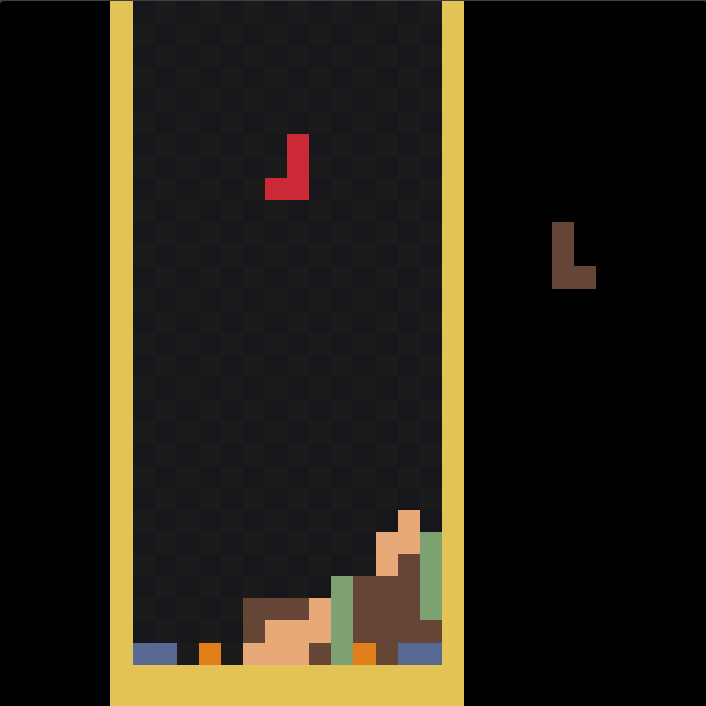
\includegraphics[width=0.3\textwidth]{game_screenshot.png}
    \caption{Screenshot of the game}
    \label{Instructions}
\end{figure}

\item Game Summary:
% TODO: Tell us a little about your game.
\begin{itemize}
\item The game is like the traditional tetris, where the player can control (move left, right, down, rotate) each tetromino. When tetromino drop to the bottom, a new tetromino will be generated from the top.
\end{itemize}

    
\end{enumerate}

\section{Attribution Table}
% TODO: If you worked in partners, tell us who was 
%       responsible for which features. Some reweighting 
%       might be possible in cases where one group member
%       deserves extra credit for the work they put in.

\begin{center}
\begin{tabular}{|| c | c ||}
\hline
 Student 1 (Wenzhu Ye - 1005714247) &  Student 2 (Dongnuo Wu - 1009614794) \\ 
 \hline
 draw game border & fix the problem with the registers\\
 \hline
 draw game grid & implement the S key\\
 \hline
 draw single tetromino & implement the A, D key\\ 
 \hline
 generate random tetromino & implement the gravity\\ 
 \hline
 rotation of tetromino & remove the line if the line is full\\
 \hline
 detect collision of singel tetromino with wall and other landed pieces & detect whether the tetromino is landed and store it \\  
 \hline
\end{tabular}
\end{center}

% TODO: Fill out the remainder of the document as you see 
%       fit, including as much detail as you think 
%       necessary to better understand your code. 
%       You can add extra sections and subsections to 
%       help us understand why you deserve marks for 
%       features that were more challenging than they
%       might initially seem.


\end{document}
